
\documentclass[a4 paper,12pt]{article}
\usepackage[inner=2.0cm,outer=2.0cm,top=2.5cm,bottom=2.5cm]{geometry}
\usepackage{setspace}
\usepackage{appendix}
\usepackage[rgb]{xcolor}
\usepackage{tabu}
\usepackage{multirow}
\usepackage{longtable}
\usepackage{graphicx}
\usepackage{verbatim}
\usepackage{longtable}
\usepackage{subcaption}
\usepackage{fancyhdr}
\usepackage[colorlinks=true, urlcolor=blue, linkcolor=blue, citecolor=blue]{hyperref}
\usepackage{booktabs}
\usepackage{amsmath,amsfonts,amsthm,amssymb}
\usepackage{setspace}
\usepackage{fancyhdr}
\usepackage{lastpage}
\usepackage{tikz}
\usepackage{listings}
%\lstset{
	%	commentstyle=\color{red!50!green!50!blue!50},%代码块背景色为浅灰色
	%	rulesepcolor= \color{gray}, %代码块边框颜色
	%	breaklines=true,  %代码过长则换行
	%	numbers=left, %行号在左侧显示
	%	numberstyle= \small,%行号字体
	%	keywordstyle= \color{blue},%关键字颜色
	%	frame=shadowbox,%用方框框住代码块
	%	basicstyle=\ttfamily
	%}
\definecolor{dkgreen}{rgb}{0,0.6,0}
\definecolor{mauve}{rgb}{0.9,0.1,0.4}
\definecolor{ash}{rgb}{0.8,0.8,0.8}
\lstset{ 
	language=Octave,                % the language of the code
	basicstyle=\ttfamily,           % the size of the fonts that are used for the code
	numbers=left,                   % where to put the line-numbers
	numberstyle=\small\color{gray},  % the style that is used for the line-numbers
	stepnumber=2,                   % the step between two line-numbers. If it's 1, each line
	% will be numbered
	numbersep=5pt,                  % how far the line-numbers are from the code
	backgroundcolor=\color{ash},      % choose the background color. You must add \usepackage{color}
	rulesepcolor= \color{gray}, %代码块边框颜色
	showspaces=false,               % show spaces adding particular underscores
	showstringspaces=false,         % underline spaces within strings
	showtabs=false,                 % show tabs within strings adding particular underscores
	frame=single,                   % adds a frame around the code
	rulecolor=\color{black},        % if not set, the frame-color may be changed on line-breaks within not-black text (e.g. commens (green here))
	tabsize=2,                      % sets default tabsize to 2 spaces
	captionpos=b,                   % sets the caption-position to bottom
	breaklines=true,                % sets automatic line breaking
	breakatwhitespace=false,        % sets if automatic breaks should only happen at whitespace
	title=\lstname,                   % show the filename of files included with \lstinputlisting;
	% also try caption instead of title
	frame=shadowbox,%用方框框住代码块
	keywordstyle=\color{blue},          % keyword style
	commentstyle=\color{dkgreen},       % comment style
	stringstyle=\color{mauve},         % string literal style
	escapeinside={\%*}{*)},            % if you want to add LaTeX within your code
	morekeywords={*,...}               % if you want to add more keywords to the set
}
\usetikzlibrary{positioning, arrows.meta}
\usepackage{extramarks}
\usepackage{ctex,amsmath,amsfonts,amssymb,bm,hyperref,graphicx}
\usepackage{chngpage}
\usepackage{soul,color}
\usepackage{graphicx,float,wrapfig}
\newcommand{\homework}[3]{
	\pagestyle{myheadings}
	\thispagestyle{plain}
	\newpage
	\setcounter{page}{1}
	\noindent
	\begin{center}
		\framebox{
			\vbox{\vspace{2mm}
				\hbox to 6.28in { {\bf 现代电子电路基础及实验报告 \hfill} {\hfill {\rm #2} {\rm #3}} }
				\vspace{4mm}
				\hbox to 6.28in { {\Large \hfill #1  \hfill} }
				\vspace{3mm}}
		}
	\end{center}
	\vspace*{4mm}
}
\newcommand\numberthis{\addtocounter{equation}{1}\tag{\theequation}}

\begin{document}
	\homework{集成运算放大器的应用(一)}{1900011413}{吴熙楠}
	
	\section{实验目的}
	(1)通过实验了解运算放大器的基本特性;
	\par (2) 学习并掌握运算放大器的运算关系和应用;
	\par (3)了解运算放大器实现有源滤波器的方法。
	\section{实验器材}
	直流稳压电源、示波器、信号发生器、万用表、面包板 、运算放大器,电阻,电容。
	\section{实验原理}
	理想运放主要有如下特性:1.开环电压放大倍数且 $A_{VO} = \infty$;2.差模输入电阻$R_{ID}=\infty$,共模输入电阻 $R_{IC}=\infty$;3.输出电阻 $R_{o}=0	$;4.共模抑制比 $K_{CMR}=\infty$;5.输入失调电压、输入失调电流以及它们的漂移均为零。当理想运放工作在线性区,即输出电压与输入电压呈线性关系时,利用它的理想化参数可导出下面两个重要结论,即理想运放的特点:1.运放的输入电流$ i = 0$,即虚断路;2.运放的差动输入电压 $V_{+}=V_{-}=0$,即虚短路。\\
	\textbf{3.1反向比例运算}
	\begin{figure}[H]
		\centering
		\hspace{2em}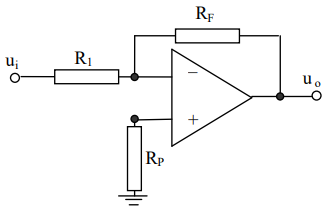
\includegraphics[width=.25\linewidth]{pic/1.png}
		\caption{\small{反向比例运算电路示意图}
		}
	\end{figure}
\par 通过计算可得:$u_{o}=\dfrac{-R_{F}}{R_{1}}u_{i}$\\
	\textbf{3.2加法比例运算}
		\begin{figure}[H]
		\centering
		\hspace{2em}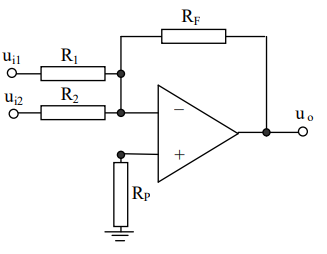
\includegraphics[width=.25\linewidth]{pic/3.png}
		\caption{\small{加法比例运算电路示意图}
		}
	\end{figure}
\par 通过计算可得:$u_{o}=-(\dfrac{R_{F}}{R_{1}}u_{i1}+\dfrac{R_{F}}{R_{2}}u_{i2})$\\
	\textbf{3.3加减比例运算}
		\begin{figure}[H]
		\centering
		\hspace{2em}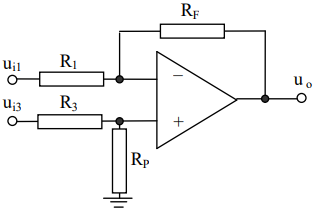
\includegraphics[width=.25\linewidth]{pic/4.png}
		\caption{\small{加减比例运算电路示意图}
		}
	\end{figure}
\par 通过计算可得:$u_{o}=-(\dfrac{R_{F}}{R_{1}}u_{i1}-\dfrac{R_{F}}{R_{3}}u_{i3})$\\
	\textbf{3.4低通滤波器}
			\begin{figure}[H]
		\centering
		\hspace{2em}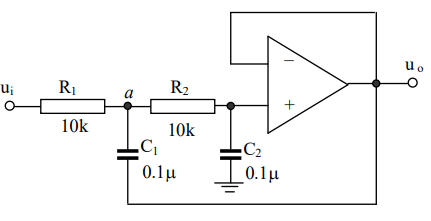
\includegraphics[width=.25\linewidth]{pic/5.png}
		\caption{\small{有源低通滤波器电路示意图}
		}
	\end{figure}
\par 通过计算可得:$f_{H}=\dfrac{\sqrt{\sqrt{2}-1}}{2\pi RC}$\\
	\textbf{3.5高通滤波器}
			\begin{figure}[H]
		\centering
		\hspace{2em}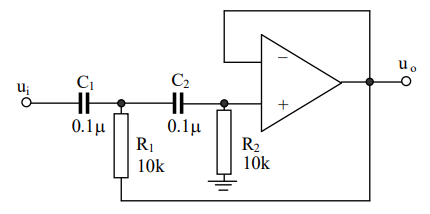
\includegraphics[width=.25\linewidth]{pic/6.png}
		\caption{\small{有源高通滤波器电路示意图}
		}
	\end{figure}
\par 通过计算可得:$f_{L}=\dfrac{\sqrt{\sqrt{2}+1}}{2\pi RC}$\\
	\section{实验内容}
\noindent
	\begin{figure}[H]
		\centering
		\hspace{2em}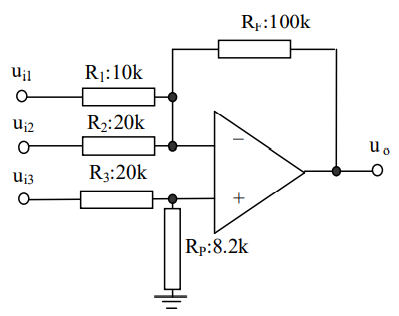
\includegraphics[width=.5\linewidth]{pic/8.png}
		\caption{\small{比例运算实验电路图}
		}
	\end{figure}
\noindent
\textbf{4.1反向比例运算电路}
\par 只有$u_{i1}$端输入信号时,在输入端加载 $f=1kHz
$的正弦信号。由实验数据可得输入电压:$u_{i}=152mV$,输出电压:$u_{o}=1.26V$。
\par 通过观察示波器上的波形图我们可知:输入输出电压的相位相反
\par 又因为$\dfrac{u_{o}}{u_{i}}=10.26\approx \dfrac{R_{F}}{R_{1}}=10$,我们也验证了反向比例电路的运算关系。
\\
\textbf{4.2加法比例运算电路}
\par $u_{i1}=u_{i2}$端输入信号时,在输入端加载 $f=1kHz
$的正弦信号。由实验数据可得输入电压:$u_{i}=152mV$,输出电压:$u_{o}=2.34V$。
\par 通过观察示波器上的波形图我们可知:输入输出电压的相位相反
\par 又因为$\dfrac{u_{o}}{u_{i}}=15.39\approx \dfrac{R_{F}}{R_{1}}+\dfrac{R_{F}}{R_{2}}=15$,我们也验证了加法比例电路的运算关系。
\\
\textbf{4.3加减比例运算电路}
\par $u_{i1}=u_{i2}=u_{i3}$端输入信号时,在输入端加载 $f=1kHz
$的正弦信号。由实验数据可得输入电压:$u_{i}=152mV$,输出电压:$u_{o}=1.58V$。
\par 又因为$\dfrac{u_{o}}{u_{i}}=10.39\approx \dfrac{R_{F}}{R_{1}}+\dfrac{R_{F}}{R_{2}}-\dfrac{R_{F}}{R_{3}}=10$,我们也验证了加减比例电路的运算关系。
\\
\textbf{4.4有源低通滤波器}
\begin{table}[H]
	\centering
	\caption{有源低通滤波器数据表}
    \resizebox{\textwidth}{!}{
	\begin{tabular}{|r|r|r|r|r|r|r|r|r|r|r|r|r|r|}
		\toprule[0.5mm]
		$f/Hz$&10&20&30&40&50&60&70&80&85&90&95&100&110\\
		\midrule
		$u_{i}/V$&1.00&1.00&1.00&1.00&1.00&1.00&1.00&1.00&1.00&1.00&1.00&1.00&1.00\\
		\midrule
		$u_{o}/V$&1.02&1.00&0.96&0.92&0.88&0.84&0.80&0.77&0.74&0.72&0.71&0.70&0.66\\
		\bottomrule[0.5mm]
	\end{tabular}}
\end{table}
	\begin{figure}[H]
		\centering
		\hspace{2em}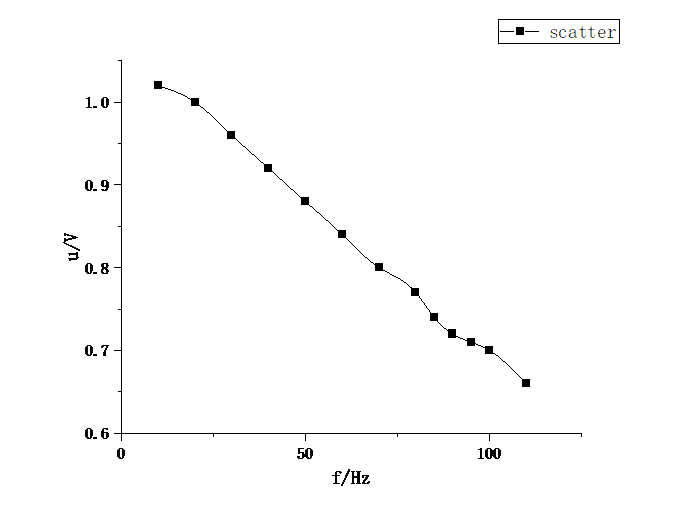
\includegraphics[width=.5\linewidth]{pic/9.png}
		\caption{\small{有源低通滤波电路幅频图}
		}
	\end{figure}
\par 由数据表可得:$f_{H}=100Hz$,理论值计算为:$f_{H}=\dfrac{\sqrt{\sqrt{2}-1}}{2\pi RC}=102.43Hz$
\\
\textbf{4.5有源高通滤波器}
\begin{table}[H]
	\centering
	\caption{有源高通滤波器数据表}
    \resizebox{\textwidth}{!}{
	\begin{tabular}{|r|r|r|r|r|r|r|r|r|r|r|r|r|r|}
		\toprule[0.5mm]
		$f/Hz$&1000&900&700&500&400&300&280&260&240&230&220&210&200\\
		\midrule
		$u_{i}/V$&1.00&1.00&1.00&1.00&1.00&1.00&1.00&1.00&1.00&1.00&1.00&1.00&1.00\\
		\midrule
		$u_{o}/V$&0.992&0.992&0.976&0.936&0.888&0.808&0.762&0.728&0.708&0.696&0.688&0.676&0.664\\
		\bottomrule[0.5mm]
	\end{tabular}}
\end{table}
	\begin{figure}[H]
		\centering
		\hspace{2em}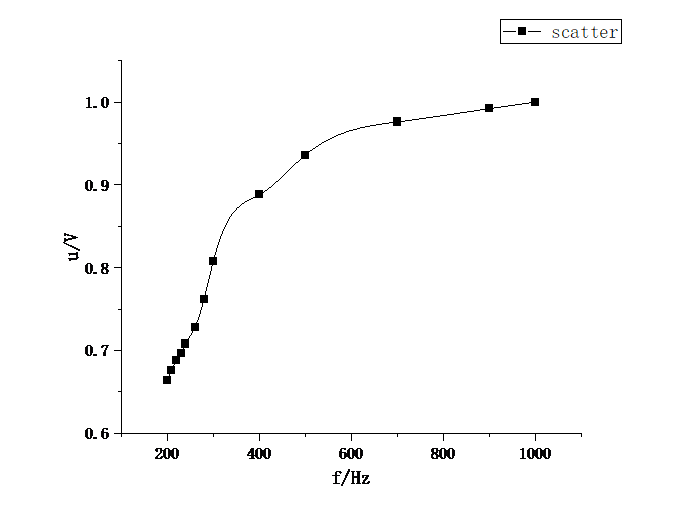
\includegraphics[width=.5\linewidth]{pic/10.png}
		\caption{\small{有源高通滤波电路幅频图}
		}
	\end{figure}
\par 由数据表可得:$f_{L}=240Hz$,理论值计算为:$f_{L}=\dfrac{\sqrt{\sqrt{2}+1}}{2\pi RC}=247.29Hz$
	\section{思考题}
	\noindent
	\textbf{1.反向运算电路的$R_{p}$有什么作用?实验过程中其值固定不变对实验结果是否有影响?为什么?
}
	\par 答:反向运算电路的$R_{p}$是电路中的平衡电阻,为了保证运放输入级差分电路的对称性,减少输入级偏置电流改变引起的运算误差,$R_{p}=R_{F}||R_{1}(A\rightarrow \infty)$;因为本次实验中$R_{p}=8.2k\Omega$,刚好能够满足平衡电路的要求,实验过程中值固定不变对实验结果不会有影响,这是由于偏置电流流过电阻带来的误差被平衡电阻抵消了的缘故。\\
	\textbf{2.有源高通滤波器中类似有源低通滤波器,引入了正反馈,试分析引入正反馈的作用。
}
	\par 答:没有正反馈的电路$K_{u}=\dfrac{1}{\sqrt{(1-\omega^{2}C^{2}R^{2})^{2}+9\omega^{2}C^{2}R^{2}}}$,没有正反馈的阻容高通滤波器的幅频特性曲线的显著缺点是在通频带中电压传输系数的模
    随频率的升高而衰减得更厉害,但在通频带下界频附近使用正反馈环路后,提高下界频附近传输系
    数的模,达到改善其幅频特性的目的。

	\begin{appendices}
		\section{原始数据整理}
	\begin{figure}[H]
		\centering
		\hspace{2em}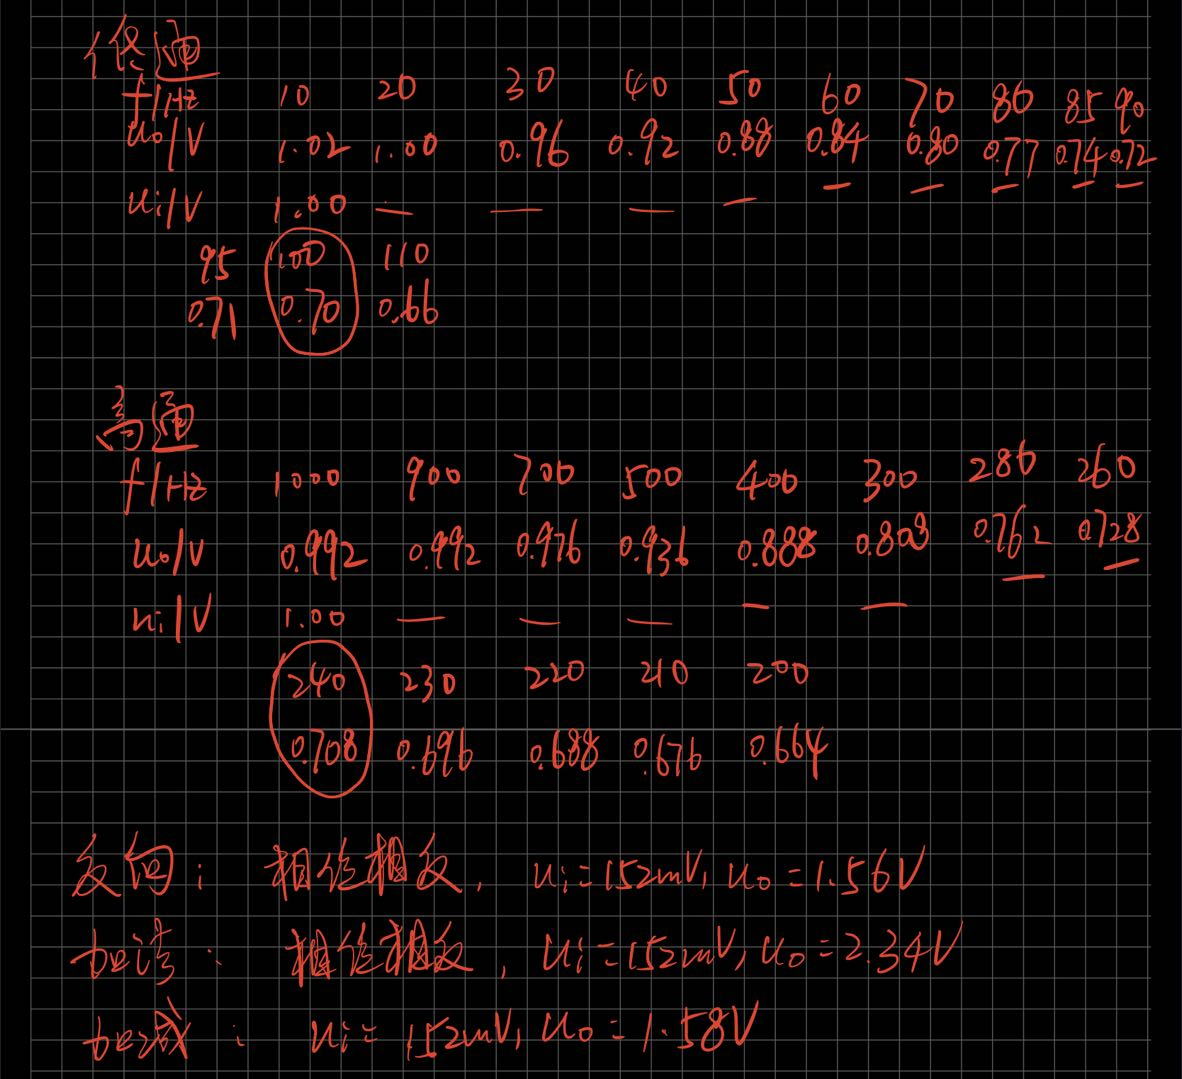
\includegraphics[width=.6\linewidth]{pic/1.jpg}
		\caption{\small{实验原始数据记录图}
		}
	\end{figure}
	\end{appendices}
\end{document} 
